\documentclass{standalone}

\usepackage[american]{circuitikz}
\usepackage{mathtools}

\begin{document}
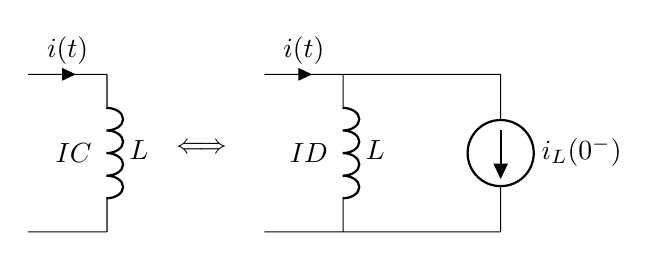
\begin{tikzpicture}
\coordinate(A) at (2.2,-1.25);
  \draw
  (0,0) to [short,-, i=$i(t)$] (1,0)
  (1,0) to [L=$L$,n=L] (1,-2) (L.s) node[left] {$IC$}
  (0,-2) to [short,-] (1,-2)
  (3,0) to [short,-, i=$i(t)$] (4,0)
  (4,0) to [L=$L$,n=L2] (4,-2) (L2.s) node[left] {$ID$}
  (6,0) to [isource, l=$i_L(0^-)$] (6,-2)
  (3,0) to [short,-] (6,0)
  (3,-2) to [short,-] (6,-2);
  \node[label=$\Longleftrightarrow$] (A) at ($(A)$) {};
\end{tikzpicture}
\end{document}